\subsection{Research Thrust 3: Behavior-guided feedback design}
\label{sec:feedback}

%\madhur{The primary intellectual merit in this section is the Deep Explanations idea as illustrated in Figure~\ref{fig:deep_exp}. The other part can be on scenario based behavior/trust modeling- but that can be part of the experiment plan too.}
%The purpose of this research thrust is to develop and validate models to quantify trust of a driver in an autonomous vehicles.
The purpose of this research thrust is to develop and validate what feedback should the autonomous vehicle provide to the passengers.
If we detect the passengers are in distress, or confused about the car's driving behavior and actions, then providing appropriate feedback and meet their emotional and behavioral needs. 
% Trust in self-driving cars is one of the big discussion points in the public debate. 
% Drivers who have always been in complete control of their car are expected to willingly hand over control and blindly trust a technology that could kill them.
% We hypothesize that trust is influenced by three components:
% \begin{enumerate}[itemsep=0pt,parsep=0pt,topsep=4pt,leftmargin=0.4in]
%     \item The person who trusts,
%     \item The system this person is supposed to trust, and
%     \item The driving situation.
% \end{enumerate}
% In addition, the first component (i.e., the person), is characterized by a certain propensity to trust, which is influenced by different factors (e.g., gender, age, opinions, character traits). This is what we want to measure in the proposed research. 
While cars have become significantly more usable — particularly with regard to reliability and safety over the past twenty years — thanks to the introduction of new technologies such as electronic fuel injection, ABS, airbags, stability control etc., many of these technologies have succeeded out-of-sight of the humans behind the wheel.
Yet when it comes to newer technologies - like advanced driver assistance systems (ADAS) , we see a much less successful integration of technology, vehicle, and user.
%Many of the technologies available in modern cars do not appear to have been developed with a particular user-centred approach. 
%They exist because the technology has become available to perform a specific function.
Furthermore, as soon as driving ``feels'' even partly autonomous, people switch off, they become disengaged from the process of driving — and fail to monitor the system, which can lead to disastrous consequences for semi-autonomous cars.
We hypothesize, that for autonomous vehicles trust comes from two factors: \textit{predictability}, and \textit{explainability}.
If a user expects a car to drive in a certain way in a certain situation, and the car conforms to his expectation, the user will tend to trust it more.
Occasionally, when the AV’s action surprise/confuse the user- as long as there is an explanation provided for it, the user can again gauge her level of trust in the system.
Given a proile of the passenger's behavior and emotional needs, from Section~\ref{sec:behaviour} the goal of this research thrust is to:
\begin{enumerate}[itemsep=0pt,parsep=0pt,topsep=4pt,leftmargin=0.4in]
    \item Develop an automated way to provide explanations for the autonomous vehicle's actions to the passenger - this caters to the \textit{explainability} aspect of a passenger's trust, and
    \item Develop user interfaces which convey the intended actions of the vehicle to the passenger so they can gauge the \textit{predictability} component of their trust in the autonomous vehicle.
\end{enumerate}



%\madhur{Madhur describes the scenario based experiments with prescan}
% feel free to create another tex input file for this subsection 
%\madhur{I will add some text to this subsection as well.}


\subsubsection{Explainability via Deep-Explanations }
\label{subsec:explainability}

\begin{figure}
    \centering
    \includegraphics[width=\columnwidth]{figures/deep_exp.pdf}
    \caption{Deep-Explanation generation: Each dimension of the scene decomposition is used as an input to caption generation. Representation matching, and seq2seq are then used to generate a likely explanation for the predominant action stream.  }
    \label{fig:deep_exp}
\end{figure}

Automatic image description generation is a challenging problem that has recently received a large amount of interest from the computer vision and natural language processing communities ~\cite{johnson2016densecap, xu2015show, wang2016image, karpathy2015deep,Vinyals2015ShowAT}
Not only must caption generation models be able to solve the computer vision challenges of determining what objects are in an image, but they must also be powerful enough to capture and express their relationships in natural language. 
For this reason, caption generation has long been seen as a difficult problem.
The task of automatic image description involves taking an image, analyzing its visual content, and generating a textual description (typically a sentence) that verbalizes the most salient aspects of the image. 
This requires the joint use of both Computer Vision and Natural Language Processing techniques.
Yet despite the difficult nature of this task, there has been a recent surge of research interest in attacking the image caption generation problem. In particular, deep neural networks have been shown to form new grammatically correct sentences as opposed to the template based models and their limited generalization capability to a novel image.
To capture the correlation between two modalities i.e. visual and natural language we need to map both these to some same space so at learn the relation between them or say we need to learn the multimodal joint model.
Models that uses different deep neural networks like convolutional neural network (CNN), long short term memory(LSTM) networks, recurrent neural network(RNN) to implicitly learn the common embedding. These by far gives the best result on all common datasets of caption generation
Aided by advances in training deep neural networks and the availability of large classification datasets, recent work has significantly improved the quality of caption generation using a combination of convolutional neural networks (convnets) to obtain vector representation of images and recurrent neural networks to decode those representations into natural language sentences.

In the proposed research we extend attention-based image caption generators to work with multidimensional data-sets.
\begin{enumerate}
    \item Instead of generating captions from RGB images alone, we will also generate captions from LIDAR data, depth sensor images, and segmented images. 
    \item The captions themselves, will be enhanced with information about the control decision (steering, acceleration, and braking) made.
    \item We will gather and release a multidimensional caption data-set specifically for autonomous vehicles. 
\end{enumerate}




\subsubsection{Predictability via user interface design}
\label{subsec:uid}
This research analyzes the current scenario and future implications of autonomous driving systems, addressing the creation process of a user interface able to communicate intentions and movements of autonomous vehicle.
The ultimate goal is to increase the confidence felt by the user to this system, encourage inclusion, acceptance and all the benefits it could bring to user mobility, and emotions.
We envision a scenario in which car is not only a tool to get from point A to point B, but a complex device that receives and provides information, is connected to the network, knows traffic situation, programs maintenance, can recognize emotional states, hypothetical distractions and driver physical problems (sleep or tiredness), is able to teach the correct way to drive through feedback and, vice-versa, learning input from the driver.
\begin{wrapfigure}{r}{0.45\textwidth}
  \begin{center}
    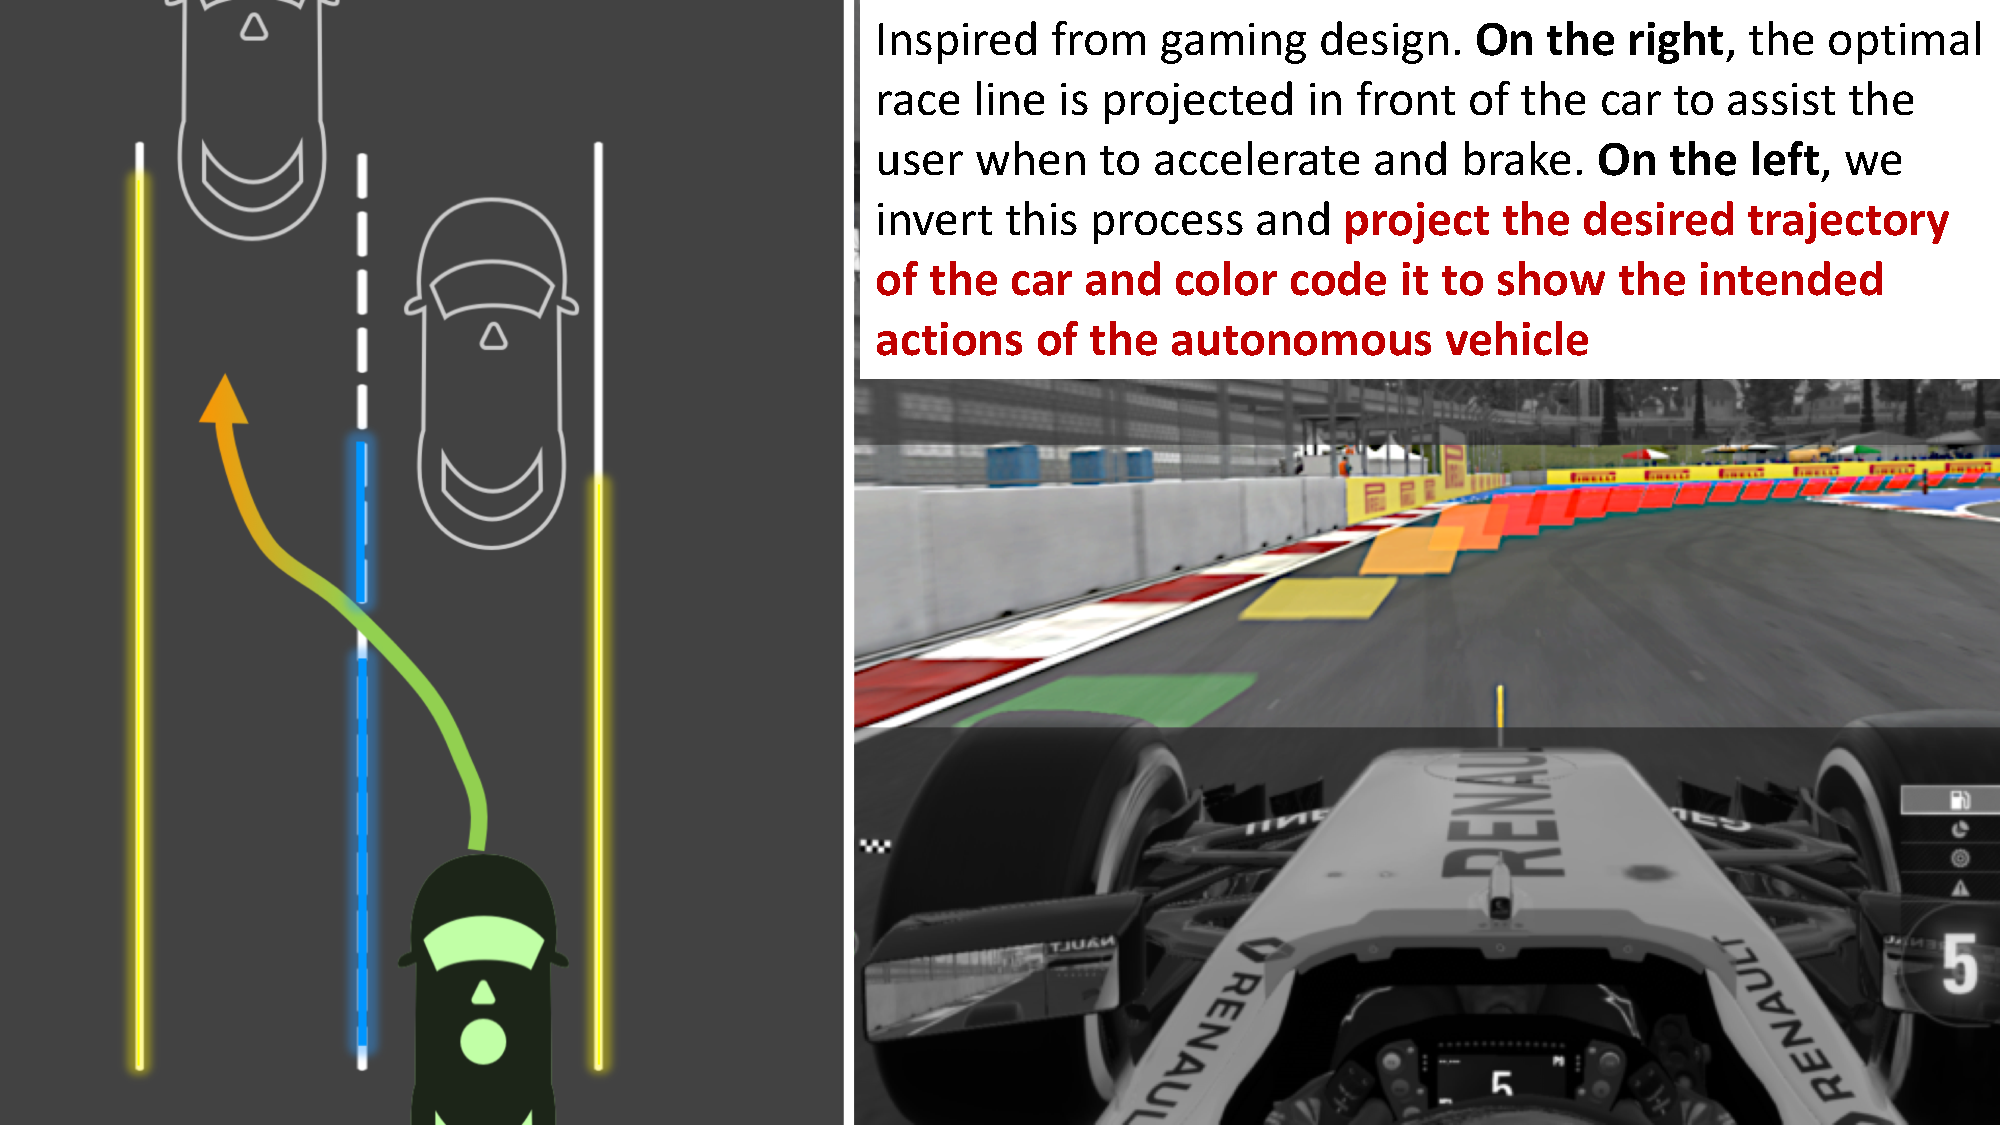
\includegraphics[width=0.43\textwidth]{figures/trajectory_ui.pdf}
  \end{center}
  \caption{Inspired from gaming, projecting the intended trajectory of the car in a color coded manner can realy critical feedback to the user about what actions the car intends to take in any given situation.}
  \label{fig:trajectory}
\end{wrapfigure}
Graphical user interface is an essential tool to create a bridge between the passenger and the autonomous vehicle. 
Present day dashboards/instrument clusters/user interface for semi autonomous vehicles present a high level overview or a wireframe view of what the car sees as its driving. Its typical to highlight lane markings and road signs, and even highlight potential hazards.
However, what is lacking is a design to transparently communicate the intended actions of the vehicle. 
Such transparency is important, because the algorithms by which autonomous cars make decisions are largely invisible to the driver.
If something unexpected occurs, the driver can only speculate what happened. In Section~\ref{subsec:explainability}, we presented an approach to explain the car's actions when driver distress, or a hard braking/steering event occurs. 

In our autonomous vehicle simulator, we will test graphical interfaces design which convey the intention of the autonomous car to the passenger. We are not proposing designing production ready user interfaces for autonomous cars, but a functional study for testing, determining visual variables complexity, information hierarchy and topology, and cognitive load for certain functional UI elements. 
Think of it as a `visual storyboard' of what is happening outside the car. The UI elements will show immediate future movements and choices. ``\textit{Why is the car turning right?}'', ``\textit{Which way is it taking?}'', ``\textit{Can the car detect the cyclist in front of me?}''.
The interface is based on two fundamental principles: simplicity (of use) and anthropomorphism (of language). 
It's not designed for an audience of engineers or designers, it is designed to be as simple as possible, usable and understandable by anyone.

To present a example, we take inspiration from design for motorsport gaming. As shown in Figure~\ref{fig:trajectory}(right), many games project a path in front of the race car to guide the user which is the fastest race line on the track. The color of the race track tells the gamer where to accelerate (green) or slow down (amber). Our idea is to invert this concept for an autonomous car where the UI (Figure~\ref{fig:trajectory}(left)) shows the intended trajectory of the autonomous vehicle and the color of the trajectory coveys if the car will speed up of slow down (brake). We hypothesize that such feedback can help passengers gauge their ``predictability'' metric and hence teir confidence, and trust in the vehicles. 


We envision that these deep explanations can offer insight into the neural networks responsible for the perception and scene understanding for self-driving cars. Such black box networks soon may also play a role in planning and control for the autonomous cars~\cite{bojarski2016end}, making it even more important to obtain explanations for their actions/predictions.
By providing readable explanations of the actions along with and correctly designed user interfaces, we provide context and feedback to the passenger, enabling an increase in the trust between the passenger and the vehicle.
The trajectories and safety regions computed in Thrust 2, will be incorporated as a part of the feedback design. 
Likewise, the explanations will be generated for instances when the emotion detection from Thrust 1 predicts the driver is confused due the the behavior of the car. 